\documentclass[a4paper,11pt]{article}
\usepackage[utf8]{inputenc}
\usepackage{amssymb}
\usepackage{amsmath} 
\usepackage{enumerate}
\usepackage{graphicx}
\usepackage{subcaption}
\usepackage{subcaption}
\graphicspath{ {./img} }
\DeclareMathOperator*{\argmax}{arg\!\max}
\DeclareMathOperator*{\argmin}{arg\!\min}
\DeclareMathOperator*{\var}{var}
\newcounter{exercise}
\setcounter{exercise}{0}
\newcounter{subexercise}
\newcommand*{\exercise}[1][]{
  \subsection*{Exercise
    \ifx/#1/\stepcounter{exercise}\arabic{exercise}
    \else#1\fi
  }
  \setcounter{subexercise}{0}
}
\newcommand*{\subexercise}[1][]{
  \par{
    \noindent\textbf{\ifx/#1/\protect\stepcounter{subexercise}\alph{subexercise}\else#1\fi.\quad}
  }
}
\title{Chapter 24}
\author{stevenjin8}
\date{\today}

\begin{document}
  \maketitle

  \section*{Exercises}

  \begin{figure}
    \begin{subfigure}{.49\textwidth}
      \centering
      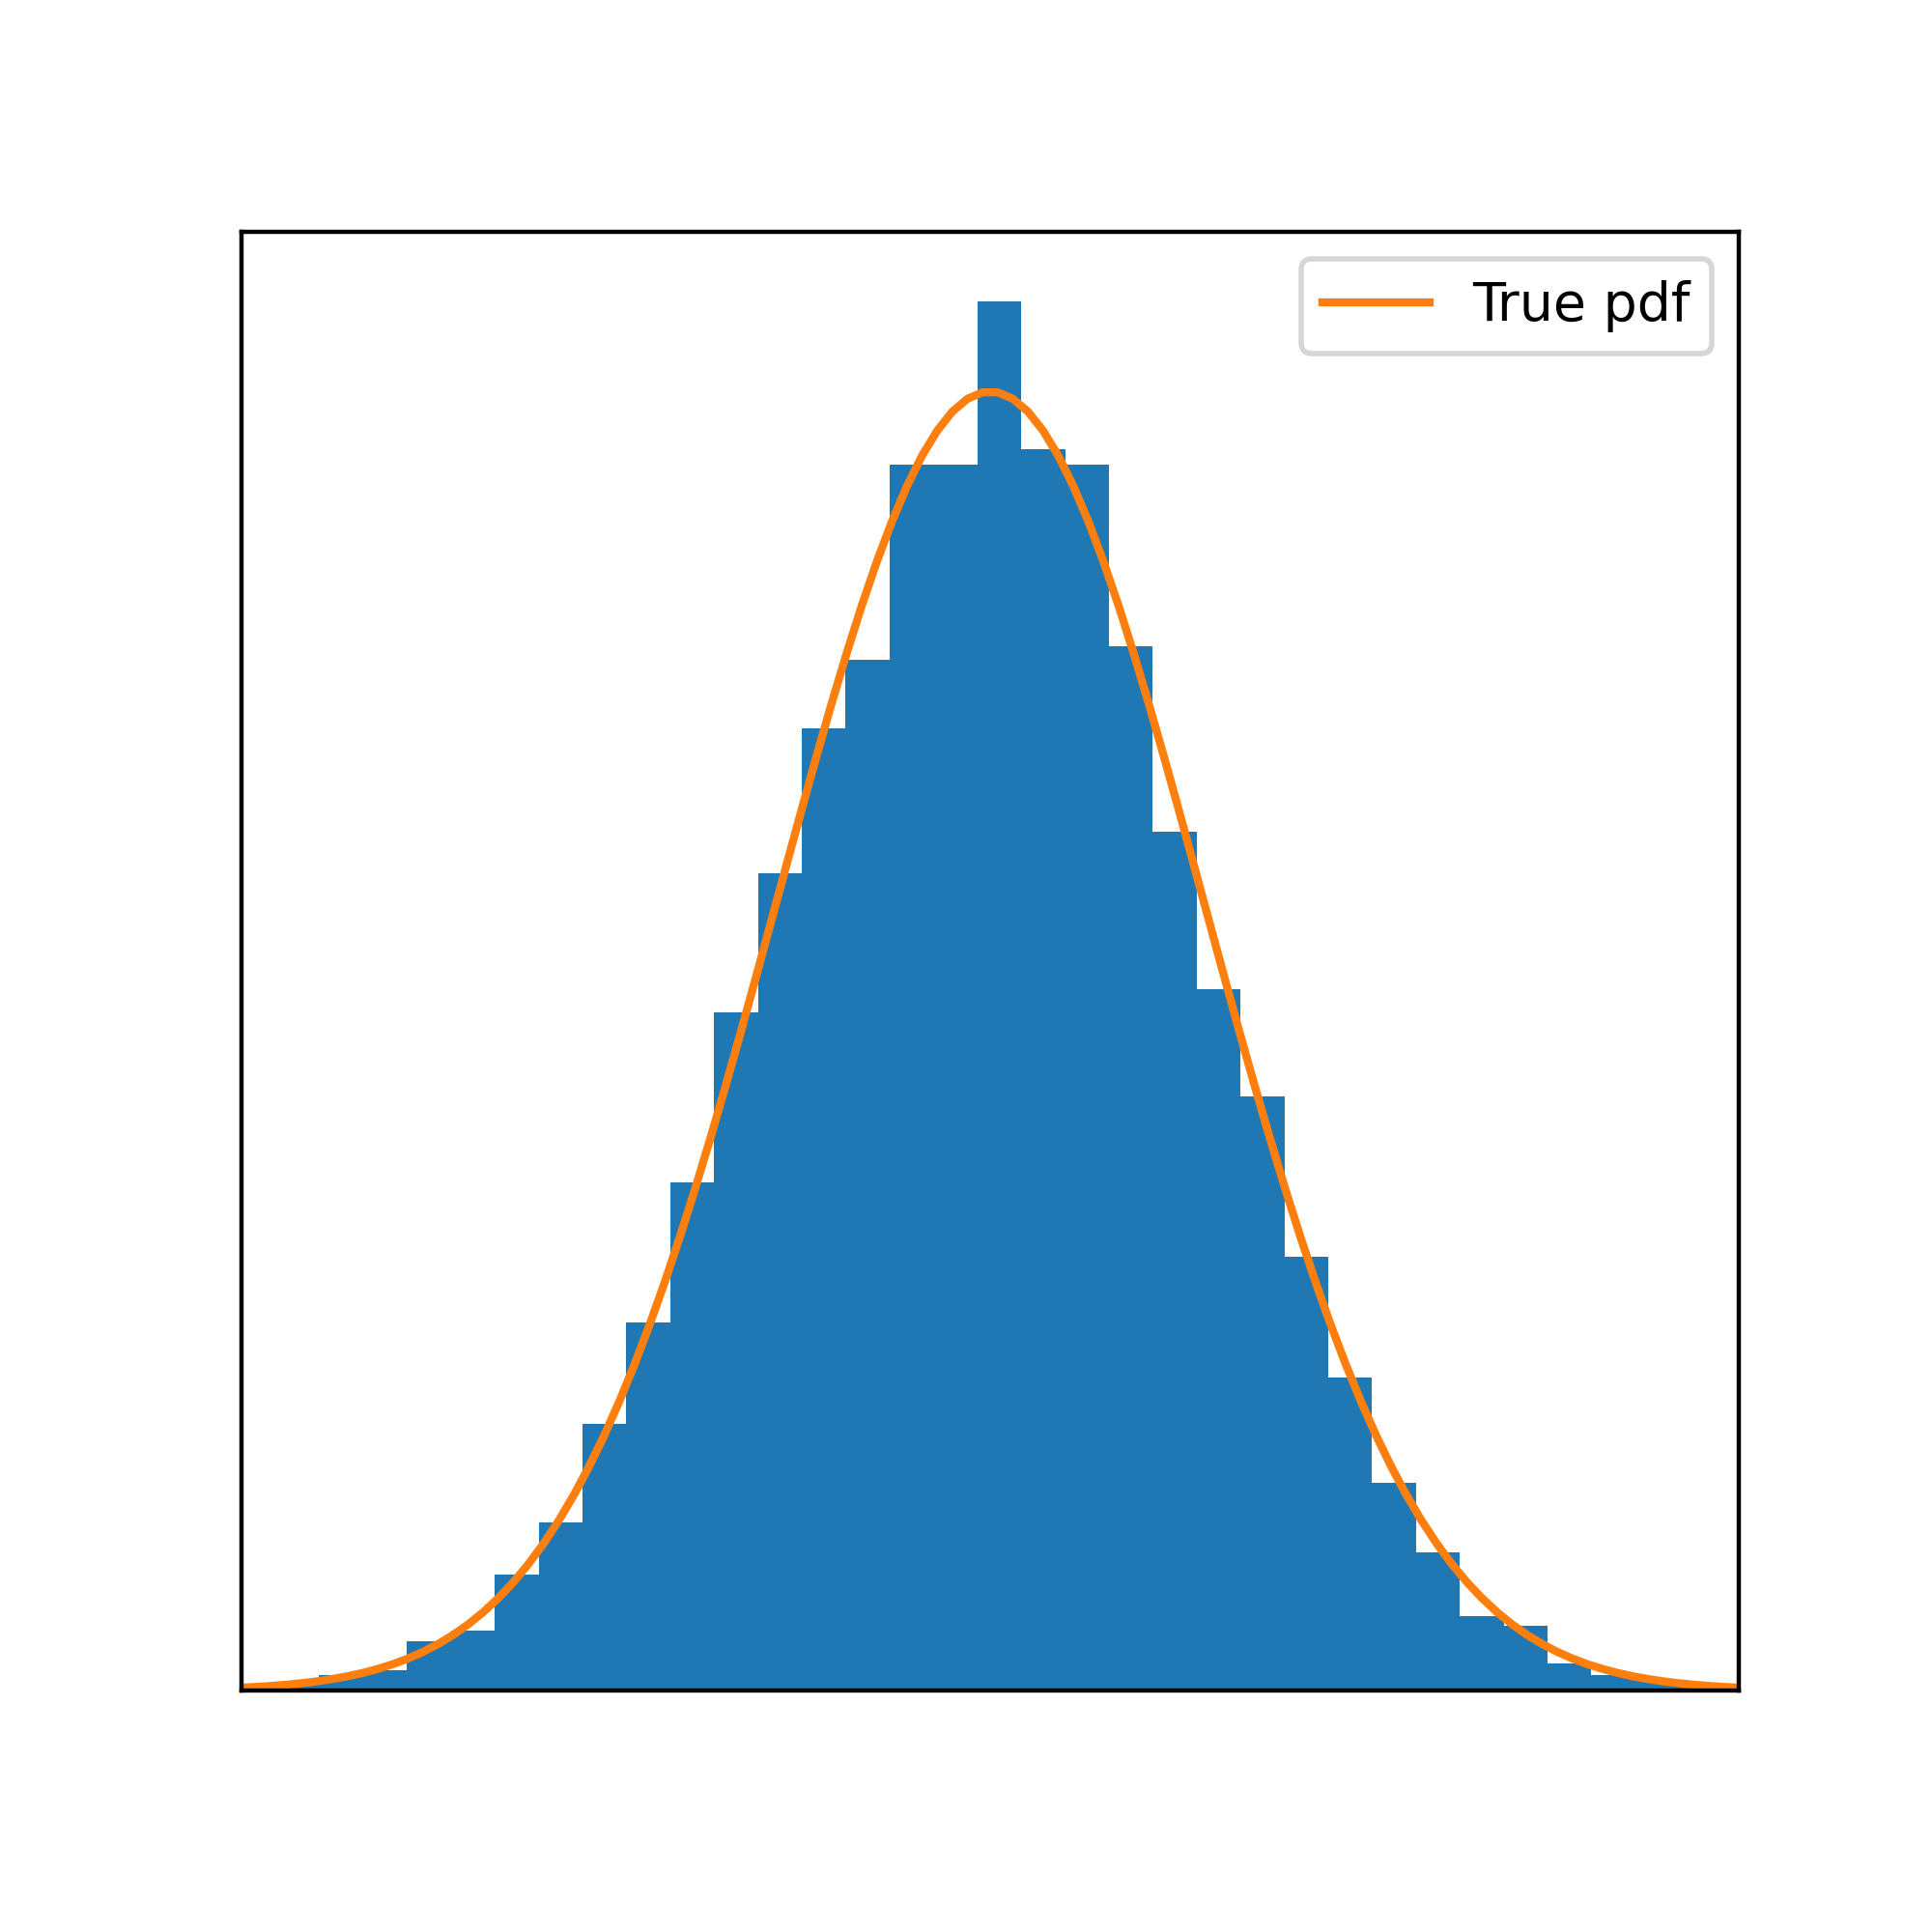
\includegraphics[width=1\linewidth]{img/gibbs/x1-hist.png}
      \caption{Empirical vs true marginal for $x_1$.}
    \end{subfigure}
    \begin{subfigure}{.49\textwidth}
      \centering
      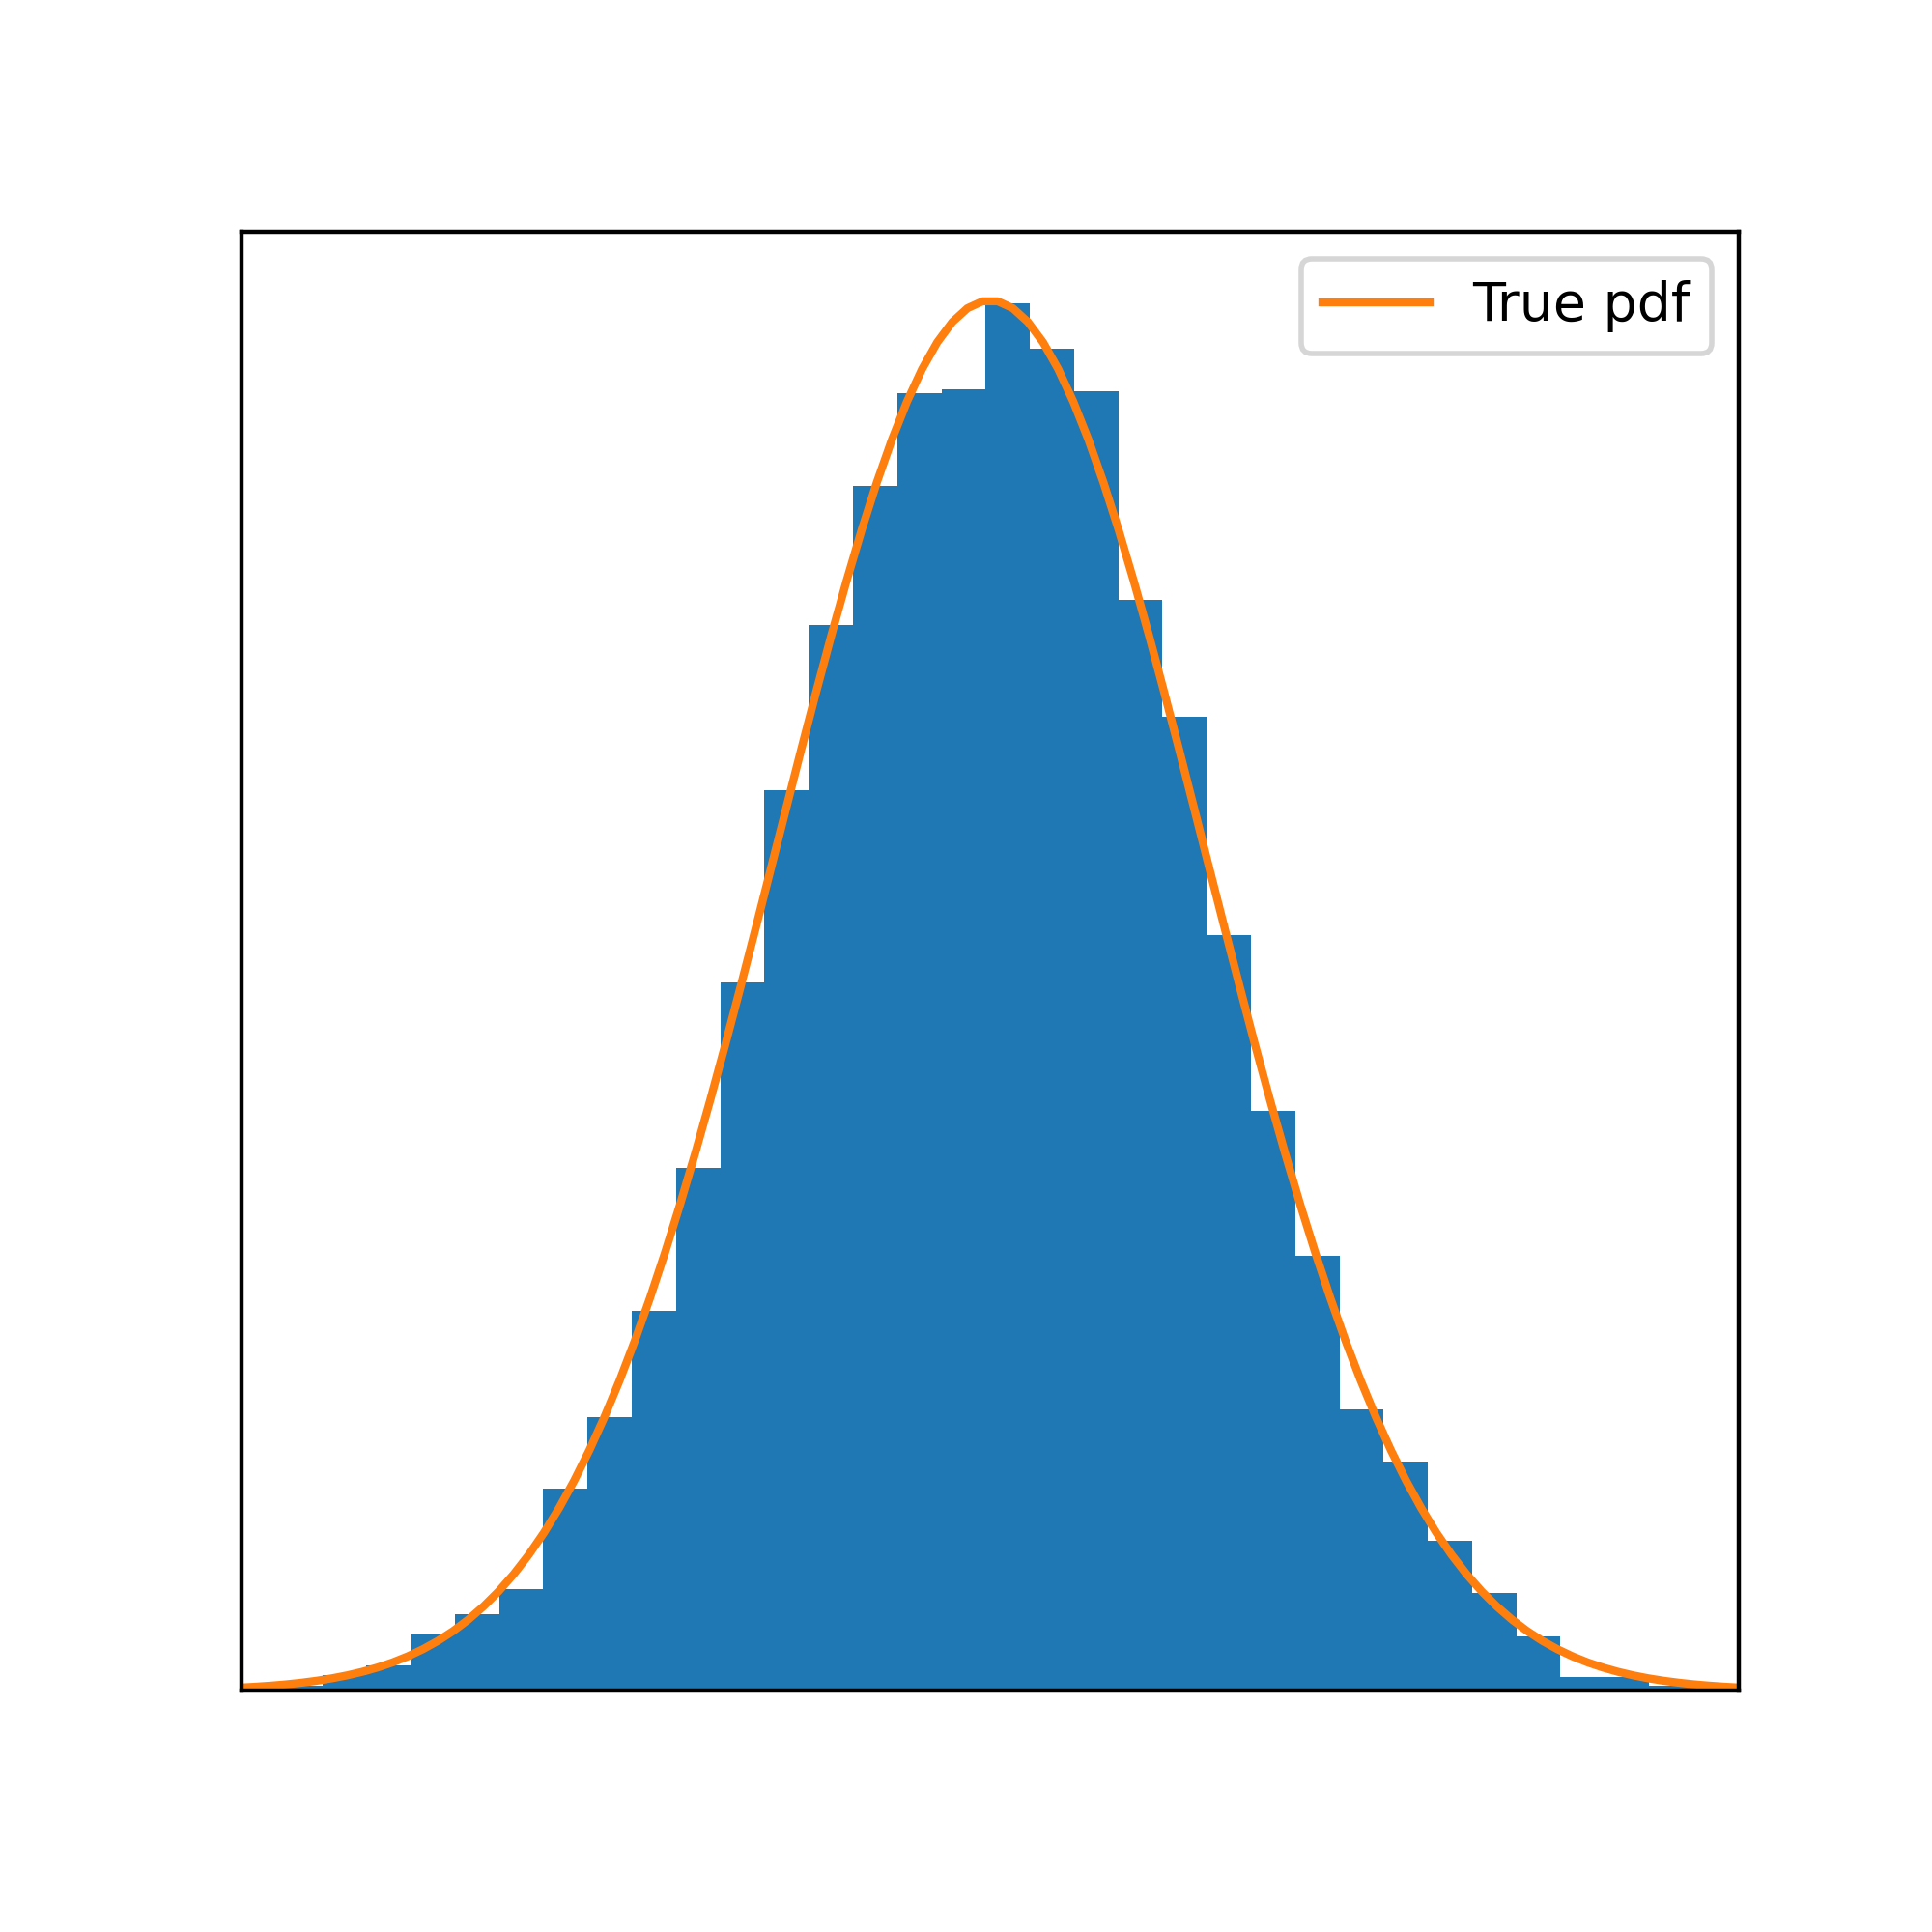
\includegraphics[width=1\linewidth]{img/gibbs/x2-hist.png}
      \caption{Empirical vs true marginal for $x_2$.}
    \end{subfigure}
    \centering
    \begin{subfigure}{.49\textwidth}
      \centering
      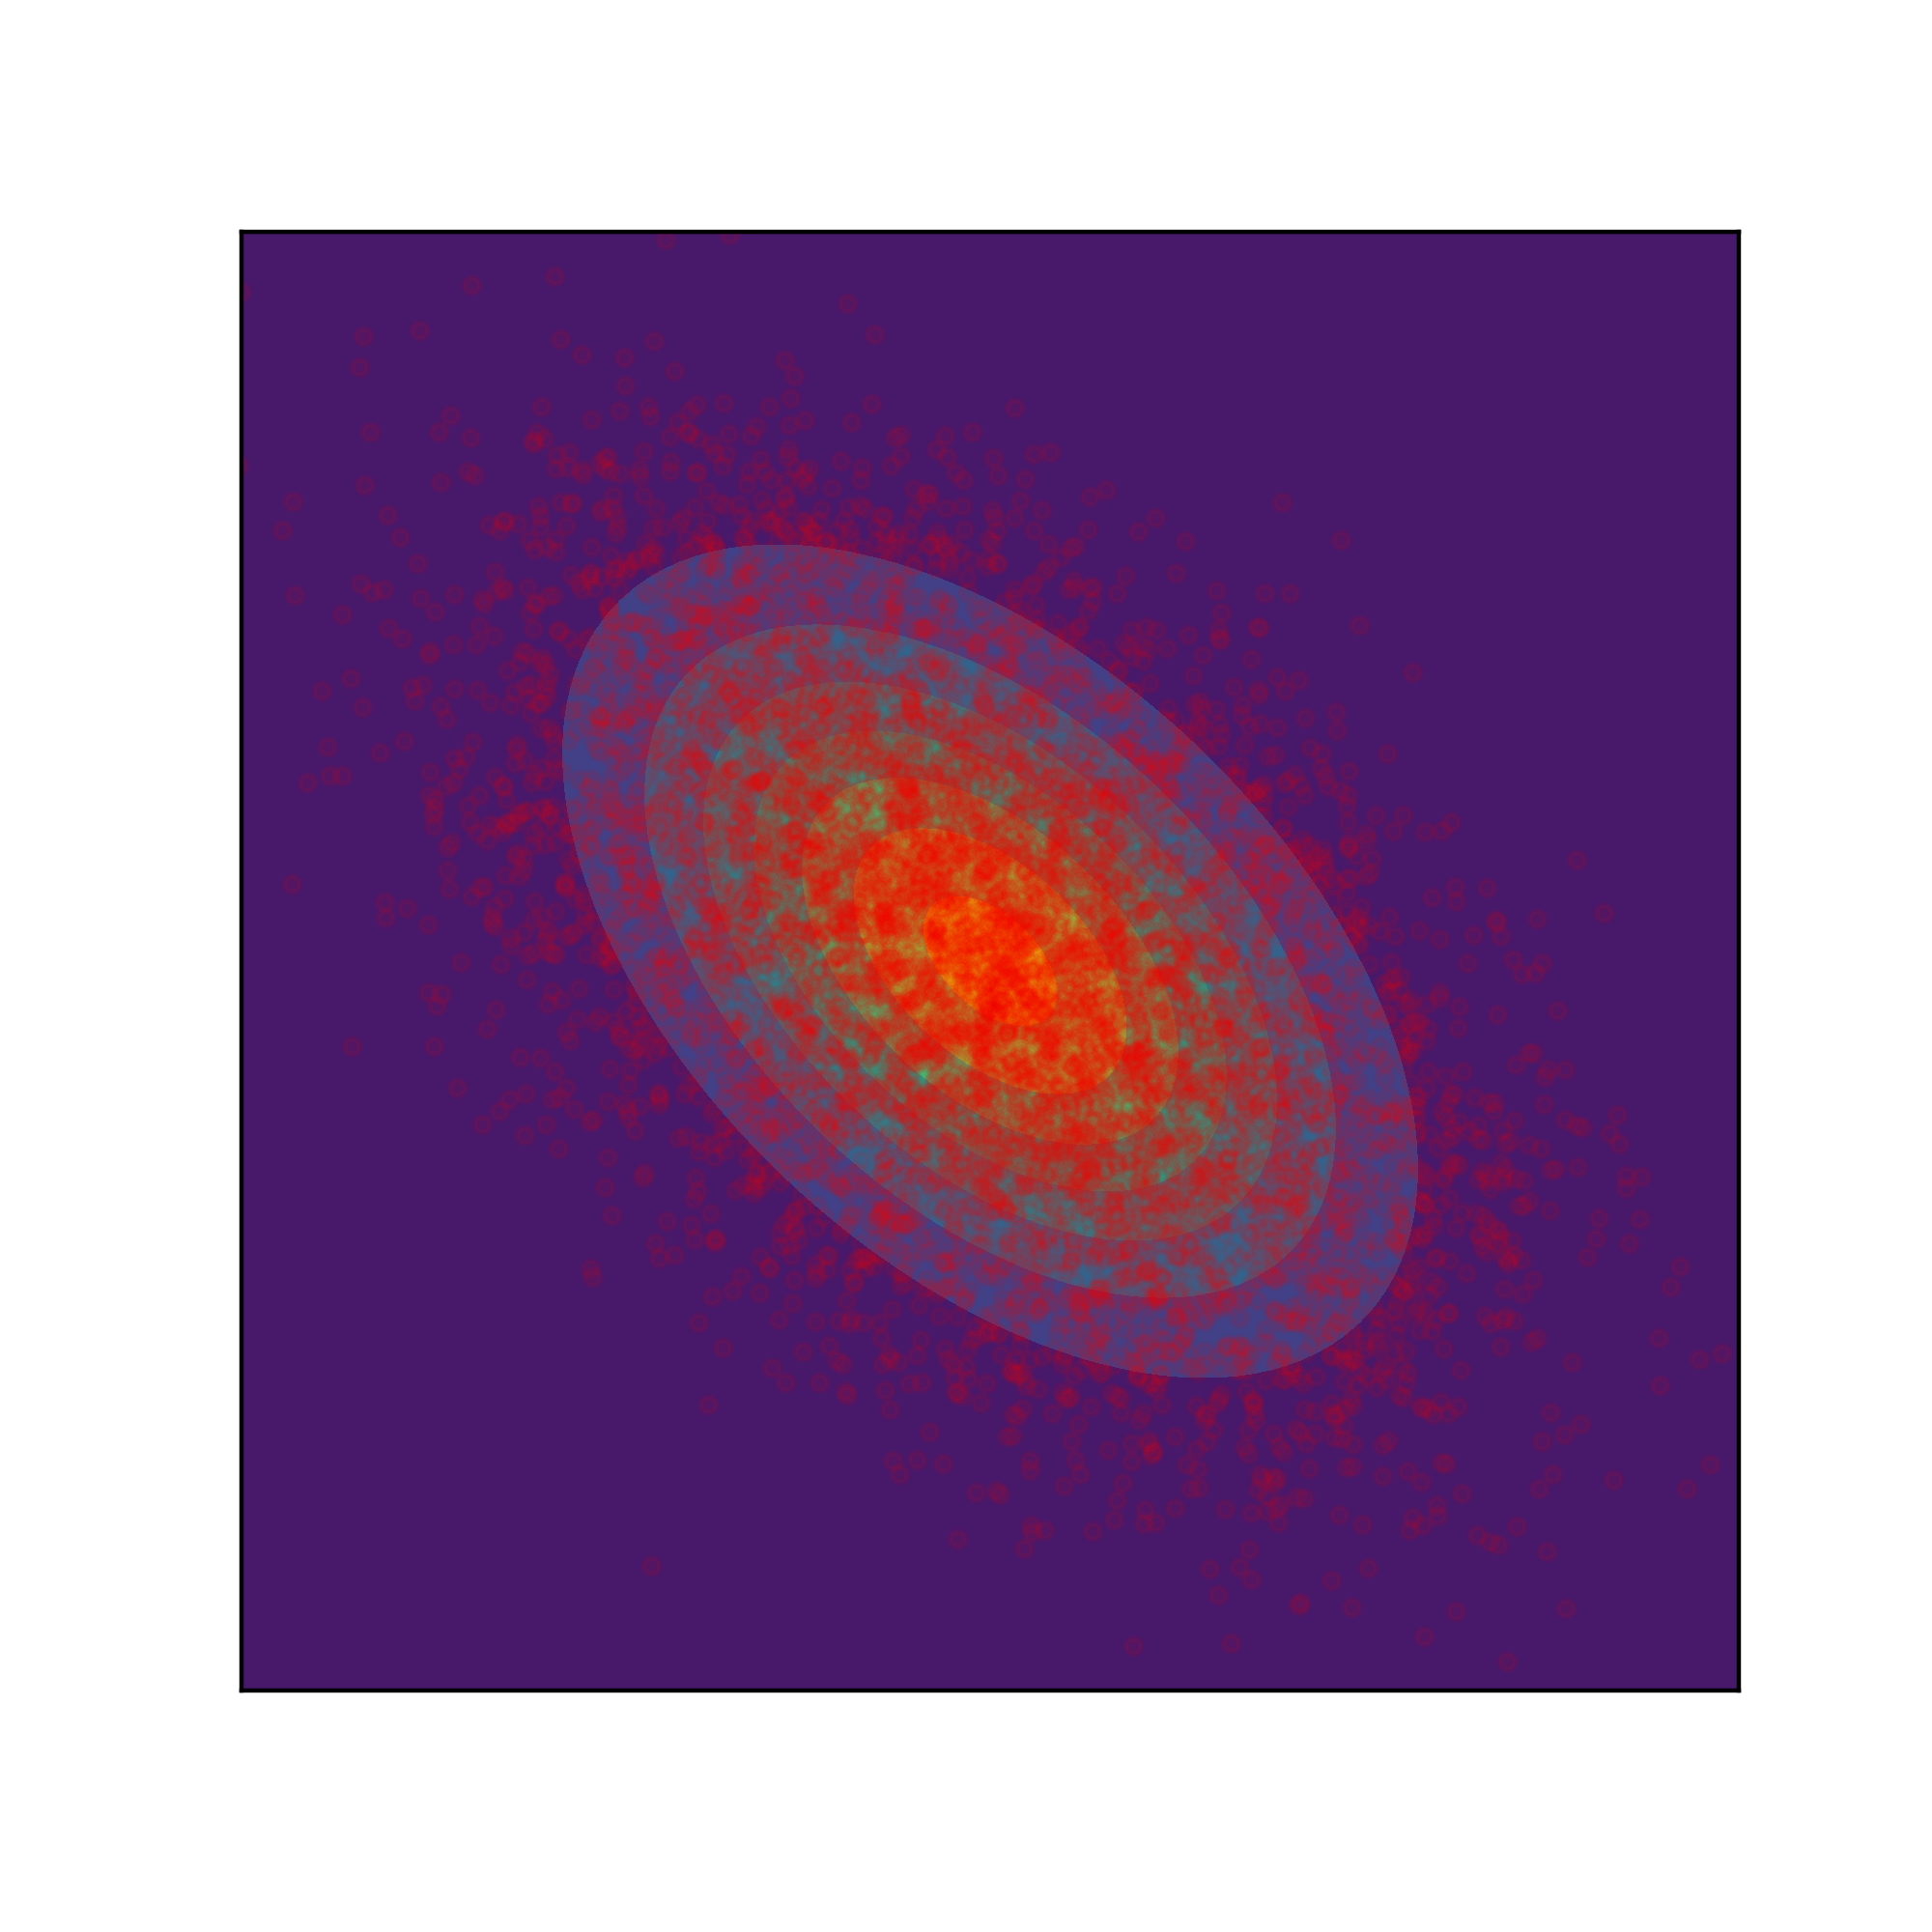
\includegraphics[width=1\textwidth]{img/gibbs/scatter.png}
      \caption{Empirical vs true marginal for $x_1, x_2$.}
    \end{subfigure}%
    \caption{Gibbs sampling a 2-D Gaussian.}
  \end{figure}


  \exercise
  \[
    p(x_1|x_2) = \mathcal{N}\left(x_1\left| \frac32 - \frac12 x_2, \frac34\right.\right)
  \]
  The formula for $p(x_2|x_1)$ is the same but with the indices switched.
\end{document}
